%!TEX program = xelatex
\documentclass[11pt,dvipsnames,table]{beamer}
\usepackage[no-math,cm-default]{fontspec}
\usepackage{amsmath}
\usepackage{amsthm}
\usepackage{amssymb}
\usepackage{CJK}
\usepackage{comment}
\usepackage{verbatim}
\usepackage{indentfirst}
\usepackage{syntonly}
\usepackage{fancyhdr}
\usepackage{xcolor}
\usepackage{graphicx}
%\usepackage{paralist}
\usepackage{beamerthemesplit}
\usepackage{euler}
\usepackage{ulem}
\usepackage{listings}
\usepackage{zhspacing}
\usepackage{booktabs}
\usepackage{multirow}
\usepackage{supertabular}
%\usepackage{mathptmx}

\usetheme{Berlin}
\usecolortheme{beaver}
\usefonttheme{professionalfonts}
%\setbeamerfont{section in toc}{size=\Large}
%\setbeamerfont{normal text}{size=9pt}
%\setbeamertemplate{headline}{}
%\setbeamertemplate{footline}{}

\defaultfontfeatures{Mapping=tex-text}
\zhspacing
%\setromanfont{Times New Roman}
\newfontfamily\zhfont[BoldFont=Adobe Heiti Std]{Adobe Song Std}
\setmonofont[Scale=1]{Courier New}
\XeTeXlinebreaklocale "zh"
\XeTeXlinebreakskip = 0pt plus 1pt

\lstset{language=C++,
	extendedchars=false,
	basicstyle=\ttfamily\footnotesize,
	keywordstyle=\bfseries\color{blue},
	identifierstyle=\color{blue!60!black},
	commentstyle=\itshape\color{gray},
	escapeinside=`'}

\setlength{\parindent}{2em}
\setlength{\baselineskip}{1.3\baselineskip}
%\linespread{1.3}

\setbeamercolor{math text}{fg=black}
\setbeamertemplate{qed symbol}{ $ \square $ }
\setbeamerfont{headline}{size=\fontsize{7.5pt}{\baselineskip}}
\setbeamerfont{footline}{size=\fontsize{7.5pt}{\baselineskip}}
\setbeamertemplate{theorems}[numbered]
\renewcommand{\thetheorem}{\arabic{subsubsection}.\arabic{theorem}}
\renewcommand{\thelemma}{\arabic{subsubsection}.\arabic{lemma}}
\renewcommand{\appendixname}{结语}

\begin{document}

\title[CodeChef题目选讲]{\fontsize{20pt}{\baselineskip}CodeChef题目选讲}
\author[THU~CST~~胡泽聪]{THU~CST~~胡泽聪\\ Email:~huzecong@163.com}
\institute[THU~CST~~胡泽聪]{}
\date{}

\maketitle

{\fontsize{10pt}{\baselineskip}

\section{Introduction}
	\subsection{About the problems}
	\begin{frame}
		\frametitle{关于题目}
		为照顾各个层次的选手,讲义中的题目分为了四类。
		\begin{itemize}
			\item Warmup。大家都能想出来的热身题。
			\item Average。比热身题稍难的一般题。
			\item Intermediate。有一定难度的进阶题。
			\item Hard。具有挑战性的难题。
		\end{itemize}
		
		每个部分内的题目按照个人主观感受的难度排序。
	\end{frame}


\section{Warmup}
	\subsection{June Challenge 2013 - Little Elephant and Mouse}
	\begin{frame} % 707
		\frametitle{LEMOUSE}
		有一个$n\times m$的格子,有一头大象,初始时在$(1,1)$,要移动到$(n,m)$,每次只能向右或者向下走。有些格子中有老鼠,如果大象所在的格子和某个有老鼠的格子的曼哈顿距离$\leq1$,大象就会被那只老鼠吓到。求一条移动路径,使得吓到过大象的老鼠数量最少。
		
		$n,m\leq100$。
	\end{frame}
	\begin{frame}
		\frametitle{LEMOUSE - Solution}
		如果多次经过一只老鼠旁边也会被吓多次,直接DP就好了。而这里只会被吓一次,我们需要往状态中加点东西。 \pause
		
		注意到,一只老鼠最多能影响我们三步,因此只要记录上两步的走法即可。转移时分情况讨论。
	\end{frame}
	
	\subsection{September Challenge 2013 - Merciless Chef}
	\begin{frame} % 191
		\frametitle{MLCHEF}
		有一棵$n$个点的有根树,$1$号节点为根,每个点有一个正点权。有$m$次操作,操作有下面两种:
		\begin{itemize}
			\item 将一棵子树内的所有点的点权减去某个正整数。
			\item 询问一棵子树内有多少个点的点权为正数。
		\end{itemize}
		
		$n,m\leq100000$。
	\end{frame}
	\begin{frame}
		\frametitle{MLCHEF - Solution}
		既然是子树操作,先求出DFS序。问题就变成了区间操作的序列问题。 \pause
		
		分块套平衡树显然可做,但是复杂度略高(还不能调\texttt{set})。有更简单的做法吗? \pause
		\vskip 1em
		由于每次减去的都是正整数,一个数变成非正数后就不会再变回正数。
		
		线段树维护区间内有多少个正数,同时维护区间最小值。当最小值$\leq0$时,就把这个数改成正无穷,同时更新区间正数个数。
		
		复杂度$O(n\log n)$。
	\end{frame}

\section{Average}
	\subsection{January Challenge 2014 - Meteor}
	\begin{frame} % 336
		\frametitle{METEORAK}
		一个$n\times m$的网格中,有$k$个坏点。有$q$次询问,每次给定$L_i$和$R_i$,询问在网格的第$L_i$到第$R_i$行中最大的内部没有坏点的矩形的面积。
		
		$n,m\leq1000$,$k\leq n\times m$,$q\leq10^6$。
	\end{frame}
	\begin{frame}
		\frametitle{METEORAK - Solution}
		令$f(L,R)$代表询问$(L,R)$的答案,令$g(L,R)$代表矩形上下边界为$L$和$R$的最大矩形宽度,显然有
		\[f(L,R)=\max(g(L,R)\times(R-L+1), f(L+1,R), f(L,R-1))\]
		问题就在于怎么求出$g(L,R)$。
	\end{frame}
	\begin{frame}
		\frametitle{METEORAK - Solution}
		一个暴力做法是,把$L\sim R$行压缩成一行,然后变成一维的问题。利用单列的前缀和,可以做到单次操作$O(n)$。\pause
		\vskip 1em
		如何优化?直接压位!单次就变成了$O(n/32)$。已经可以通过了。 \pause
		
		但是还能更优吗? \pause
		\vskip 1em
		考虑求最大全$0$子矩阵的传统$O(n^2)$做法。枚举下边界之后,求出每列向上拓展的最大高度。
		
		用单调队列可以求出,以一列的最大高度向左向右拓展,可以拓出的最大长度。设此时的高度为$h$,可以用这个长度来更新$g(R-h+1\sim R, R)$。
		
		用树状数组之类的数据结构可以做到$O(n^2\log n)$,直接打标记之后扫一遍可以做到$O(n^2)$。
	\end{frame}
	
	\subsection{March Lunchtime 2014 - A Game With a Sheet of Paper}
	\begin{frame}
		\frametitle{SHGAME}
		一张$n\times m$的网格,其中某个格子$(x,y)$被涂黑了。两个玩家轮流操作,每次沿一条水平或竖直的格线将网格切成两部分,并舍弃不含黑格子的一部分。无法操作者败。
		
		双方均以最优策略行动。问有多少种$(x,y)$的选择使得先手必胜。
		
		$n,m\leq 10^6$,100组测试数据。
	\end{frame}
	\begin{frame}
		\frametitle{SHGAME - Solution}
		我们固定住$(x,y)$,然后考虑切一刀造成的影响。 \pause
		
		可以发现,如果我们切$(x,y)$上方,则显然其上方的行数会减少,但其左右列数及下方行数不变。如果我们分别记上下左右的行(列)数为$u,d,l,r$,则一次操作相当于将一个变量减去一个不大于其自身的数,其他变量不变。
		
		这其实就是一个4堆石子的Nim游戏。 \pause
		
		那么一个朴素的做法就是枚举$(x,y)$,然后判断$u,d,l,r$的异或和是否为0,若不为零则先手必胜。
	\end{frame}
	\begin{frame}
		\frametitle{SHGAME - Solution}
		但这样显然太慢了。
		
		一个(显然)的观察是,$u+d=n-1$,$l+r=m-1$。 \pause
		
		这意味着$u\textrm{ xor }d$与$l\textrm{ xor }r$的值分别是$O(n)$和$O(m)$级别的。 \pause
		
		我们只需预处理$u\textrm{ xor }d=u\textrm{ xor }(n-1-u)$的所有取值,并计算每种取值的个数。接下来枚举$l$,只要$u\textrm{ xor }(n-1-u)\neq l\textrm{ xor }r=l\textrm{ xor }(m-1-l)$,这一选择就合法。故可以用总方案数$n\times m$减去不合法方案数,即异或值相同的方案数。
		
		复杂度为$O(n+m)$。
	\end{frame}
	
	\subsection{August Challenge 2013 - Sereja and Ballons}
	\begin{frame} % 265
		\frametitle{SEABAL}
		一排有$n$个数,初始均为$0$。给定$m$个区间,有$k$次操作,每次会将一个数改成$1$,并询问此时有多少个给定区间中所有数均为$1$。
		
		$n,m\leq100000$,强制在线。
	\end{frame}
	\begin{frame}
		\frametitle{SEABAL - Solution}
		将一个数改为$1$后,可能会将两个分开的全$1$区间合并到了一起。第一步要做的就是找出这个区间。可以用并查集维护向左和向右的位置。 \pause
		
		记上面找到的左右端点为$L$和$R$。接下来的问题就是,找出所有在加入前还不全为$1$,加入后就全为$1$的区间。这些区间一定满足左右端点在$[L,R]$中,且并未在之前被删除。我们只需要快速找到这些区间,并删除即可。 \pause
		
		这是一个二维查询,很容易想到用线段树套平衡树实现。内层的平衡树可以用\texttt{set}。
		
		复杂度$O(n\log^2n)$。
	\end{frame}
	\begin{frame}
		\frametitle{SEABAL - Extras}
		如果没有强制在线,有更好的做法吗?
		\vskip 1em
		欢迎大家讨论。
	\end{frame}
	
	\subsection{May Lunchtime 2014 - Brand New Game}
	\begin{frame} % 265
		\frametitle{BNGAME}
		有一排$n$个格子,从左到右编号为$1\sim n$。第$i$个格子中有两个数$a_i$和$b_i$。玩家初始时站在所有格子左边(0号格子),每次移动玩家可以前进$1\sim k$个格子,并在停下的那个格子落子。当玩家移出所有格子,即到达$n$号格子右边时,游戏结束。
		
		设落子的格子为$S=\{p_1,\ldots,p_{|S|}\}$,则一盘游戏的得分为
		\[\max_{x\in S}(a_x)+\max_{y\in S}(b_y)\]
		求最小得分。
		
		$n\leq 500000$,$|a_i|,|b_i|\leq 32000$。
	\end{frame}
	\begin{frame}
		\frametitle{BNGAME - Solution}
		朴素做法是枚举$\max(a_x)$,禁止所有$a_i$大于枚举值的格子,并动态规划求出只使用剩下的格子能取到的最小的$\max(b_y)$。这样的复杂度为$O(nW)$,其中$W=\max\{a_i,b_i\}$。 \pause
		\vskip 1em
		记枚举的$\max(a_x)=K$,并记此时的$\max(b_y)=f(K)$。显然随着$K$增加,$f(K)$单调不增。
		
		如果要使$f(K)$减少,那么我们不能在任意$b_i=f(K)$的格子中落子,也即,禁止所有这样的格子后仍然可以到达终点。
		
		从小到大枚举$K$,每次$K$增加,就会有原来被禁止的格子取消禁止。此时我们尝试逐个禁止$b_i=f(K)$的格子,如果能全部禁止,则说明$f(K)$可以减小,并对减小后的$f(K)$重新尝试禁止。 \pause
		
		如何快速判断可以到达终点?
	\end{frame}
	\begin{frame}
		\frametitle{BNGAME - Solution}
		我们只需要知道,需要禁止的点的前一个和后一个未被禁止的点之间,是否能通过一步移动到达。 \pause
		
		使用平衡树维护位置即可。可以直接用STL中的set。
	\end{frame}

\section{Intermediate}
	\subsection{December Challenge 2013 - Lucy and the Flowers}
	\begin{frame}
		\frametitle{DECORATE} % 93
		给定字符串$S$,选择$S$的$n$个回文子串(可以相同)构成一个序列。如果两个序列经过旋转和/或翻转后相同,则认为两个序列同构。如,序列$\{$\texttt{"ab"}$,$\texttt{"a"}$,$\texttt{"b"}$\}$与序列$\{$\texttt{"a"}$,$\texttt{"ab"}$,$\texttt{"b"}$\}$同构。
		
		求有多少种本质不同的序列。
		
		$n\leq600$,$|S|\leq100000$。
	\end{frame}
	\begin{frame}
		\frametitle{DECORATE - Solution}
		我们可以把问题分为两个子问题:
		\begin{itemize}
			\item 求出$S$有多少本质不同的回文子串。记这个值为$x$。
			\item 求出用$x$种不同的颜色给长度为$n$的序列染色,有多少种本质不同的方案。
		\end{itemize}
	\end{frame}
	\begin{frame}
		\frametitle{DECORATE - Solution}
		先来解决第二个子问题。 \pause
		\vskip 1em
		根据Burnside引理,本质不同的着色数等于各置换下不动点的平均数。
		
		这里一共有$2n$种置换。由于$n$很小,可以暴力计算出每个置换的循环个数。
		
		对于一个有$k$个循环的置换,其不动点个数就是$x^k$。
	\end{frame}
	\begin{frame}
		\frametitle{DECORATE - Solution}
		第二个问题被轻松愉快地解决了,再来看看第一个问题。 \pause
		\vskip 1em
		由于回文子串的数量可以达到$O(n^2)$,所以我们需要高效的算法。 \pause
		
		先考虑一个与之相关的问题。求出一个字符串有多少回文子串的最快的算法是什么? \pause
		
		Manacher算法! \pause
		
		而一个字符串的本质不同回文子串只会是Manacher算法在向右拓展时的子串,因此本质不同的回文子串的个数是$O(n)$的。 \pause
		
		不过这里面还是可能有相同的子串。怎么办呢? \pause
		
		Hash一下不就完了吗?
	\end{frame}
	\begin{frame}
		\frametitle{DECORATE - Solution}
		结合这两个算法,我们就得到了这道题的最终算法。
		
		子问题一算法的复杂度为$O(|S|\log|S|)$(因为要排序去重)。
		
		子问题二算法的复杂度为$O(n^2)$。
		
		总复杂度为$O(|S|\log|S|+n^2)$。
		
		顺带一提这题要高精度。
	\end{frame}
	
	\subsection{February Challenge 2014 - Little Elephant and Movies}
	\begin{frame}	% 258
		\frametitle{LEMOVIE}
		对于一个序列,定义其``激动值''为序列中严格大于前面所有数的元素的个数。比如,$\{1,1,5,6,5\}$的激动值为$3$。
		
		给定$n$个数$p_1,p_2,\ldots,p_n$,求这$n$个数的所有排列中,激动值不超过$k$的个数。
		
		$1\leq k\leq n\leq 200$,$1\leq p_i\leq200$。
	\end{frame}
	\begin{frame}
		\frametitle{LEMOVIE - Solution}
		先记录相同的数的个数,然后去重。 \pause
		
		从大到小考虑每组相同的数。令$f[i][j]$代表已经插入前$i$大的数,且激动值为$j$的序列方案数。 \pause
		
		考虑当前这组数插入在哪些位置。每一组数的贡献至多为$1$,有贡献当且仅当至少一个数被插在了最前面。无论插入在什么位置,已有的激动值不会减少。 \pause
		
		假设已经插入了$x$个数,当前这组有$y$个数,没有一个数被插在最前面的方案数为
		\[y!\binom{x+y-1}{x-1}\]
		至少一个被插在最前面的可以类似算。
		
		复杂度$O(nk)$。
	\end{frame}
	\begin{frame}
		\frametitle{LEMOVIE - Extras}
		如果激动值的定义为,序列中相邻的且构成逆序对的数对呢?
		
		(为啥会有这个问题,是因为我最开始就把题目看成这个了) \pause
		
		这个问题实际上稍难于原问题。 \pause
		\vskip 1em
		做法类似。从小到大考虑,此时插入一个数可能会抵消之前的激动值。枚举有几个数插在原来的非逆序对之间,可以类似地算出方案数。
		
		复杂度$O(nk^2)$。
	\end{frame}
	
	\subsection{July Cook-Off 2014 - Tree Again}
	\begin{frame} % 439
		\frametitle{RRTREE2}
		给定$n$个点的有根树,1号点为根,每个节点有权值$w_i$。我们称一个数$S$合法,当且仅当存在一个$1\sim n$的排列$p$,使得$p$为这棵树的某个DFS序列,且存在$1\leq k\leq n$使得
		\[\sum_{i=1}^{k}{w_{p_i}}=S\]
		
		对于所有$1\leq S\leq \sum{w_i}$,判断$S$是否合法。
		
		$n\leq 500$,$\sum{w_i}\leq 100000$。
	\end{frame}
	\begin{frame}
		\frametitle{RRTREE2 - Solution}
		从特殊情况入手:假设树的深度为1,即除了根节点之外都是叶子节点。 \pause
		
		此时问题可以简化为01背包问题。 \pause
		
		考虑原问题,假设我们凑出$S$时在$x$节点。此时必须和可以被加进背包的有哪些东西? \pause
		
		必须被加进去的是从$x$到根路径上的所有点;可以被加进去的是$x$及祖先的所有兄弟的\textbf{整棵子树}。
	\end{frame}
	\begin{frame}
		\frametitle{RRTREE2 - Solution}
		我们在DFS的过程中处理完一个点时,就把它所有儿子的子树中所有节点权值之和视为一个物品,加进背包;在往下DFS的时候,把选择的儿子的子树权值和对应的物品从背包中删除。接下来就可以递归处理了。
		
		如何从背包中删除物品?\pause
		
		存储方案数,对多个数取模。\pause
		
		由于每棵子树只会被加入一次删除一次,故总复杂度为$O(nW)$,其中$W=\sum{w_i}$。\pause
		\vskip 1em
		有没有更加优美的做法呢?
	\end{frame}
	\begin{frame}
		\frametitle{RRTREE2 - Solution}
		当然是有的。我们要求的只是:$n$个物品删去每一个分别得到的背包。 \pause
		
		可以考虑分治:每次处理删去前一半中物品的背包,将后一半物品依次加入前一半的背包。反之亦然。
		
		这样每个物品会被加入$O(\log{s})$个背包中,其中$s$为其兄弟个数。
		
		故总复杂度为$O(nW\log n)$。
	\end{frame}
	
	\subsection{June Challenge 2013 - Just Some Permutations 3}
	\begin{frame} % 439
		\frametitle{PERMUTE}
		求有多少个$1\sim n$的排列满足,任意相邻的两个数之和不超过$m$。
		
		$2\leq n\leq1000000$,$n<m<2n$,有$100000$组测试数据。
	\end{frame}
	\begin{frame}
		\frametitle{PERMUTE - Solution}
		考虑从大到小插入所有数字。考虑插入一个数字时,其左边和右边相邻的数字是什么。
		
		对于最开始的状态,可行的数字是$1,2,\ldots,m-n$,以及左右端点。我们可以选择两个数字,或者一个端点和一个数字。 \pause
		
		插入之后,我们把$n$以及两边的数字(或端点)看做一个整体,记作$s(n)$。显然,这个整体也可以与之后的任意数字相邻。那么我们从此时的可行集合中删去这次选择的两个数字(或端点),再插入$s(n)$和$m-n+1$。这就是下一步的可行集合。可以发现可行集合的大小没有变。 \pause
		
		而当插入到$\lceil\frac{m}{2}\rceil$时,就可以任意排列了。此时尚未确定位置的就是可行集合中的元素个数。当$m$为偶数时,方案数是$(m-n)!$;当$m$为奇数时,方案数是$(m-n+1)!$。
	\end{frame}
	\begin{frame}
		\frametitle{PERMUTE - Solution}
		令$f(n,k)$为可行集合大小为$k$(这里忽略端点)时,填入$n$到1的方案数。我们有
		\begin{eqnarray*}
			f(n,k) & = & k(k-1)f(n-1,k)+2k\cdot f(n-1,k) \\
			 & = & k(k+1)f(n-1,k) \\
			 & = & (k(k+1))^if(n-i,k)
		\end{eqnarray*}
		前面的部分是选择两个数字,后面则是选择一个端点和一个数字。 \pause
		
		因此答案就是
		\[f(n,m-n)=\left\{
			\begin{array}{ll}
				(k(k+1))^{n-\left\lceil\frac{m}{2}\right\rceil}(m-n)! & m\textrm{ is even} \\
				(k(k+1))^{n-\left\lceil\frac{m}{2}\right\rceil}(m-n+1)! & m\textrm{ is odd}
			\end{array}
		\right.\]
	\end{frame}
	
	
\section{Hard}
	\subsection{December Challenge 2013 - Query on a tree IV}
	\begin{frame}
		\frametitle{QTREE6} % 64
		给定一棵$n$个点的树,每个点可以是黑色或者白色。初始时所有点都是黑色。有$m$次操作,操作有下面两种:
		\begin{itemize}
			\item 询问有多少个节点与$u$相连。两个节点$u$和$v$相连当且仅当$u$到$v$的路径上所有点(包括$u$、$v$两点)的颜色相同。
			\item 改变节点$u$的颜色。
		\end{itemize}
		
		$n,m\leq100000$。
	\end{frame}
	\begin{frame}
		\frametitle{QTREE6 - Solution}
		一个比较棘手的地方在于,修改影响的点可能有儿子、祖先甚至没有祖先与子孙关系的节点。 \pause
		
		如果只询问子树中相连的节点有多少个,要怎么做呢? \pause
		\vskip 1em
		维护黑白两种颜色的答案。修改时查询子树的答案,然后将所有相连的祖先的答案都减去这棵子树的答案。
		
		找到最浅的相连祖先,就变成了链修改问题。
		
		而查询就直接是点查询。 \pause
		\vskip 1em
		如何找最浅的相连祖先? \pause
		
		维护到根路径上的黑点个数,倍增时查询。
		
		还是只要链修改和点查询。
	\end{frame}
	\begin{frame}
		\frametitle{QTREE6 - Solution}
		我们需要一个支持链修改和点查询的数据结构。 \pause
		
		动态树显然可以,但还有更简单的方法。 \pause
		
		用轻重链剖分的思想,在DFS的时候先走重链。这样得到的DFS序列中重链会是一个区间。
		
		一条链也就会被划分成$O(\log n)$个区间。链修改就成了区间修改。
		
		树状数组即可胜任。
	\end{frame}
	\begin{frame}
		\frametitle{QTREE6 - Solution}
		回到最开始的问题。 \pause
		
		其实问题已经解决了对吧?
		
		因为一个点的答案就是其最浅相连祖先的子树的答案。
		
		直接套用上面的方法就可以解决了。
		\vskip 1em
		总复杂度为$O(n\log^2n)$,瓶颈在于倍增部分。
		
		如果有同学对于如何优化到$O(n\log n)$有想法,欢迎在课后来讨论。
	\end{frame}
	
	\subsection{February Challenge 2014 - Count on a Treap}
	\begin{frame}	% 12
		\frametitle{COT5}
		Treap是一棵平衡树,每个点有两个值,key和weight。Treap的形态使得key值满足BST的性质,且weight值满足堆的性质。
		
		维护一个大根堆Treap,有$n$次操作,操作有下面三种:
		\begin{itemize}
			\item 插入一个key值为$k$,weight值为$w$的节点。
			\item 删除key值为$k$的元素。
			\item 查询Treap中key值为$k_u$和$k_v$的元素在Treap中的距离。这里距离定义为树上两个点之间唯一路径的长度。
		\end{itemize}
		
		$n\leq200000$,任意两个点的key值和weight值均不相同。
	\end{frame}
	\begin{frame}
		\frametitle{COT5 - Solution}
		Treap期望$O(\log n)$的复杂度来源于weight值的随机性。如果weight值随机,那么期望树高也是$O(\log n)$级别的,我们完全可以暴力。
		
		但题目中weight值是给定的,Treap可以被构造成一条链,我们不能直接建立一棵Treap来模拟操作。
		
		我们需要挖掘Treap特别的性质。
	\end{frame}
	\begin{frame}
		\frametitle{COT5 - Solution}
		我们可以把问题分成两个部分:
		\begin{itemize}
			\item 求出两个点的LCA。
			\item 求出一个点的深度。
		\end{itemize}
		解决了这两个问题,就可以回答询问了。
	\end{frame}
	\begin{frame}
		\frametitle{COT5 - Solution}
		先考虑如何求出两个点的LCA。 \pause
		\vskip 1em
		设两个点为$u$和$v$,不妨设$k_u<k_v$。设其LCA为$x$。 \pause
		
		有这样一个结论:$k_u\leq k_x\leq k_v$。可以用反证法证明。 \pause
		
		而由Treap的堆的性质可得,$x$应该是key值在$[k_u,k_v]$内且weight值最大的元素。
		
		因此,我们只需要一个支持动态RMQ的数据结构,即可找到LCA。
	\end{frame}
	\begin{frame}
		\frametitle{COT5 - Solution}
		再考虑如何求出一个点的深度。设需要求深度的点为点$x$。 \pause
		\vskip 1em
		一个点的深度即其不同的祖先的个数。结合上面求LCA的算法,我们有一个暴力的想法:
		
		枚举所有其他的点,和$x$求LCA,看有多少个不同的LCA。
		
		直接这么做肯定不行,我们想想可不可以优化这个方法。 \pause
		
		这个方法等价于,固定区间的一个端点,另一个端点扫过所有的数,问最大值变化了几次。 \pause
		
		我们如果把另一个端点从固定的端点开始移动,会发现这个变化次数实际上就是,从固定的端点向左向右看,比之前的所有数字都大的数的个数。
		
		而这个问题是可做的,我们分开考虑左右两个方向的答案,实际上这个问题就是2012年集训队清华集训的《楼房重建》。
	\end{frame}
	\begin{frame}
		\frametitle{COT5 - Solution}
		《楼房重建》要怎么做? \pause
		\vskip 1em
		线段树套平衡树?应该是能做的,但是细节特别多(我写到一半就放弃了)。 \pause
		
		事实上,我们可以只用线段树完成这个任务。 \pause
		\vskip 1em
		很明显,满足条件的数是单调递增的。我们修改一个数只会对后面的数字造成影响。
		
		考虑线段树划分出来的若干个区间,有两种情况:
		\begin{itemize}
			\item 区间中的最大值小于等于修改的数。显然这个线段的贡献为$0$。
			\item 否则,我们将这个区间分成两部分。如果左侧的最大值大于修改的数,那么是不影响右侧的贡献的,只需递归处理左侧;否则又变成了第一种情况,只需递归处理右侧。
		\end{itemize}
		
		单次操作的复杂度为$O(\log^2n)$。
	\end{frame}
	\begin{frame}
		\frametitle{COT5 - Solution}
		实现上的伪代码大致如下:
		
		{\noindent
		\begin{figure}[h!]
			\centering
			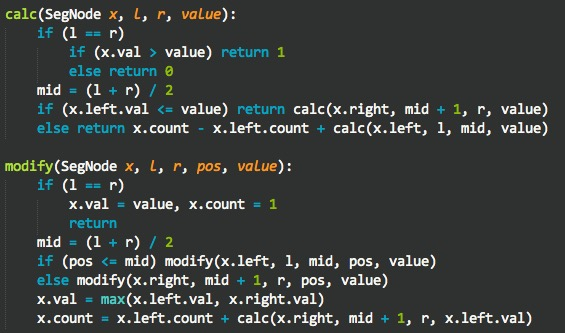
\includegraphics[width=8cm]{code.png}
		\end{figure}
		}
	\end{frame}	
	\begin{frame}
		这里\texttt{x.count}为,仅考虑\texttt{x}代表的区间时,比前面所有数都大的数的个数。注意\texttt{calc}函数中最后一个\texttt{return}那里的实现。
		
		查询类似,此处从略。
	\end{frame}
	\begin{frame}
		\frametitle{COT5 - Solution}
		回到原问题。
		\vskip 1em
		由于问题没有强制在线,我们可以先读入所有操作,无视删除,处理出最后的排好序的key值序列。这样插入和删除操作都可以视为weight值的修改,插入即改为应有的weight值,删除则改为$0$。 \pause
		
		那么两部分都可以用线段树完成了。总复杂度$O(n\log^2 n)$。 \pause
		\vskip 1em
		如果强制在线呢? \pause
		
		改成平衡树就好了。
	\end{frame}
	
\appendix
\section{}
	\begin{frame}
		\frametitle{The End}
		\centering
		\LARGE
		谢谢!
		
		欢迎课后交流!
	\end{frame}
}

\end{document}
